\section{Trees}
\emph{Connected acyclic graphs where two vertices are connected by only one path, with $|V| - 1$ edges in total.}

\subsection{Binary Search Trees}
\emph{A tree which is either empty or has \code{left} and \code{right} children binary trees.}

The \textbf{binary search tree property} states that all keys in the \code{left} sub-tree are less than the parent key,
and all keys in the \code{right} subtree are greater than the parent key.

The \textbf{height} of a BST is the number of edges on the longest path from the root to the leaf:\\[-0.2em]
\[ h(\code{v}) = \begin{cases} 
    0 & \text{if $v$ is a leaf} \\
    -1 & \text{if $v$ is null} \\
    \max(h(\code{v.left}), \; h(\code{v.right})) + 1 & \text{otherwise} \\
 \end{cases}
\]

The \textbf{minimum} and \textbf{maximum} keys are found by traversing the left and right subtrees respectively.

\textbf{Searching} for a specific key is done by comparing the key with the parent key,
recursively searching \code{v.left} if less than, \code{v.right} if greater than, and stopping if equal.

\textbf{Inserting} is akin to searching, but instead adding a new node at a leaf.

\textbf{Deleting} is trivial if if the node to be deleted has one or no children.
Otherwise, the node to be deleted is replaced by the minimum of the right subtree (its successor):

\begin{lstlisting}[
    mathescape,
    columns=fullflexible,
    basicstyle=\fontfamily{lmvtt}\selectfont,
  ]
successor(v):
    if v has a right child:
        return the minimum key in v.right
    else:
        walk up the tree to a node w
        where w.parent.left = w, or w is the root
        return w
\end{lstlisting}

All these operations are $O(h)$.
However, trees with the same keys need not have the same shape, and height depends on shape,
which is determined by insertion order.

There are $n!$ insertion orders, and $\approx 4^n$ possible shapes for a binary tree.

\subsection{AVL Trees}
\emph{Augmented BST which stores the tree height in each node.}

This augmented height field must be updated with every \code{insert} and \code{delete}.

A binary search tree is \textbf{balanced} iff $h = O(\log n)$, such that all operations take $O(\log n)$ time.

A node $v$ is \textbf{height-balanced} iff $|\code{v.left.height} - \code{v.right.height}| \leq 1$.
A height-balanced tree with $n$ nodes has height $h < 2 \log n$, and one with height $h$ has at least $n > 2^\frac{h}{2}$ nodes.

\subsubsection{Rotations}
\emph{Used to rebalance trees after insertion and deletion.\\ Left and right rotations are inverses of each other.}
\begin{center}
    \begin{forest}
        [$A_{k+2}$, red
            [$B_{k+1}$, baseline, blue
                [$L_{k}$, tier=0, roof]
                [$M_{k}$, tier=0, roof]
            ]
            [$R_{k-1}$, tier = 0, roof]
        ]
    \end{forest}
    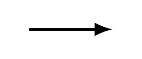
\begin{tikzpicture}
        \draw [-latex, very thick] (0,0) -- +(30pt,0);
        \end{tikzpicture}
    \begin{forest}
    [$B_{k+2}$, blue
        [$L_{k}$, tier=0, roof]
        [$A_{k+1}$, baseline, red
            [$M_{k}$, tier=0, roof]
            [$R_{k-1}$, tier=0, roof]
        ]
    ]
    \end{forest}
    \\[0.5em]Case 1: \textcolor{red}{$A$} is left-heavy but \textcolor{blue}{$B$} is balanced $\rightarrow$ right-rotate.

    \begin{forest}
        [$A_{k+2}$, red
            [$B_{k+1}$, baseline, blue
                [$L_{k}$, tier=0, roof]
                [$M_{k-1}$, tier=0, roof]
            ]
            [$R_{k-1}$, tier = 0, roof]
        ]
    \end{forest}
    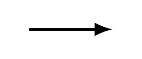
\begin{tikzpicture}
        \draw [-latex, very thick] (0,0) -- +(30pt,0);
        \end{tikzpicture}
    \begin{forest}
        [$B_{k+1}$, blue
            [$L_{k}$, tier=0, roof]
            [$A_{k}$, baseline, red
                [$M_{k-1}$, tier=0, roof]
                [$R_{k-1}$, tier=0, roof]
            ]
        ]
    \end{forest}
    \\[0.5em]Case 2: \textcolor{red}{$A$} is left-heavy but \textcolor{blue}{$B$} is left-heavy $\rightarrow$ right-rotate.

    \begin{forest}
        [$A_{k+2}$, red
            [$B_{k+1}$, baseline, tier=2, blue
                [$L_{k-1}$, roof, tier=1]
                [$C_{k}$, tier=1, magenta
                    [M1, roof]
                    [M2, roof]
                ]
            ]
            [$R_{k-1}$, roof, tier=1]
        ]
    \end{forest}
    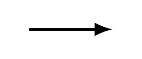
\begin{tikzpicture}
        \draw [-latex, very thick] (0,0) -- +(30pt,0);
        \end{tikzpicture}
    \begin{forest}
    [$A_{k+2}$, red
        [$C_{k+1}$, baseline, magenta
            [$B_{k}$, blue
                [$L_{k-1}$, roof, tier=0]
                [M1, roof]
            ]
            [M2, roof, tier=0]
        ]
        [$R_{k-1}$, roof, tier=0]
    ]
    \end{forest}
    \\[0.5em]Case 3: \textcolor{red}{$A$} is left-heavy but \textcolor{blue}{$B$} is right-heavy $\rightarrow$ left-rotate \textcolor{blue}{$B$},
    but \textcolor{red}{$A$} and \textcolor{magenta}{$C$} are still out of balance! M1 and M2 have a height of either $k-1$ or $k-2$.
\end{center}
\begin{center}
    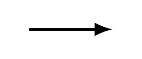
\begin{tikzpicture}
        \draw [-latex, very thick] (0,0) -- +(30pt,0);
    \end{tikzpicture}
    \begin{forest}
        [$C_{k+1}$, magenta
            [$B_{k}$, baseline, blue
                [$L_{k-1}$, roof, tier=1]
                [M1, roof, tier=0]
            ]
            [$A_{k}$, red
                [M2, roof, tier=0]
                [$R_{k-1}$, roof, tier=1]
            ]
        ]
    \end{forest}
    \\[0.5em]Case 3 (continued): Fixing the imbalance with a right-rotate about \textcolor{red}{$A$}.
\end{center}

After an \code{insert}, at most 2 rotations are needed, but \code{delete} may require up to $O(\log n)$ rotations.

This is because \code{delete} reduces height and rotations reduce height, so it is not sufficient to only fix
the lowest imbalanced node in the tree.


\subsection{Dictionary}
\emph{An abstract data type akin to a symbol table, but with support for successor and predecessor queries.}

Implemented with balanced trees.